%%%%%%%%%%%%%%%%%%%%%%%%%%%%%%%%%%%%%%%%%%%%%%%%%%%%%%%%%%%%%%%%%%%%%%
%%%%%%%%%%%%%%%%%%%%%%%%%%%%%%%%%%%%%%%%%%%%%%%%%%%%%%%%%%%%%%%%%%%%%%
\documentclass[dvips,portrait]{seminar}             %%%%%%%%%%%%%%%%%%
                                                    %%%%%%%%%%%%%%%%%%
%%%%%%%%%%%%%%%%%%%%%%%%%%%%%%%%%%%%%%%%%%%%%%%%%%%%
% gmake chi_mcan-ps
%======================



%%%%%%%%%%%%%%%%%%%%%%%%%%%%%%%%%%%%%%%%%%%%%%%%%%%%%%%
%%%%%%%%%%%%%%%%%%%%%%%%%%%%%%%%%%%%%%%%%%%%%%%%%%%%%%%
\begin{document}                     %%%%%%%%%%%%%%%%%%


%%%%%%%%%%%%%%%%%%%%%%%%%%%%%%%%%%%%%%%%%%%%%%%%%%%%%%%%%%%%%%%%%%%%%%%%%%%%%
%%%%%%%%%%%%%%%%%%%%%%%%%%%%%%%%%%%%%%%%%%%%%%%%%%%%%%%%%%%%%%%%%%%%%%%%%%%%%
%%%%%%%%%%%%%%%%%%%%%%%%%%%%%%%%%%%%%%%%%%%%%%%%%%%%%%%%%%%%%%%%%%%%%%%%%%%%%
                                                         %%%%%%%%%%%%%%%%%%%%
\begin{slide*}
\titbox{{\small\Color{Magenta} 
      ${\cal KK}$ M.C. versus semi-analytical; EEX class }}

{\bf Notation and introductory exercise, for more detailed analysis see next slides.}

{\small\Color{Blue}
  Process: $e^-e^+\to f\bar{f}$, for $f=\mu^-$, at $\sqrt{s}=$189 GeV.\\
  ISR and FSR, IFI=ISR*FSR int. off, EW off.\\
  Total x-section $\sigma(s'>s'_{\min})$ where $s'=m^2_{f\bar{f}}$.
}
\begin{center}
\setlength{\unitlength}{1mm}
%
\begin{picture}(37,37)
\put(30,30){\makebox(0,0)[lb]{\Color{Red}(a)}}
\put(-1, 0){\makebox(0,0)[lb]{
\epsfig{file=chi_mcan-O2mca.eps,width=37mm,height=37mm}
}}\end{picture}
%
\begin{picture}(37,37)
\put(30,30){\makebox(0,0)[lb]{\Color{Red}(b)}}
\put(-1, 0){\makebox(0,0)[lb]{
\epsfig{file=chi_mcan-O2dif.eps,width=37mm,height=37mm}
}}\end{picture}
%
\end{center}

{\small\Color{Red}
  (a) EEX2 ${\cal KK}$ MC confronted with the EEX2 semi-analytical results.
  The ``Z radiative return'' (ZRR) contains as much x-section as Born!\\
  (b) The difference between M.C. and semi-analytical (SAN) results.
}
\\
{\small\Color{Blue}
Notation:
\fbox{EEX2 = \Oeex{1,\alpha,\alpha L,\alpha^2 L^2}};\\
\fbox{\bf EEX} read:
{\bf E}xclusive {\bf EX}ponentiation based on Yennie Frautschi and Suura 1961,
implemented similarly as in BHLUMI, KORALZ/YFS3.
}
%-----------------------------------------------------------
\vfill
\end{slide*}   %%%
%%%%%%%%%%%%%%%%%%



%%%%%%%%%%%%%%%%%%%%%%%%%%%%%%%%%%%%%%%%%%%%%%%%%%%%%%%%%%%%%%%%%%%%%%%%%%%%%
%%%%%%%%%%%%%%%%%%%%%%%%%%%%%%%%%%%%%%%%%%%%%%%%%%%%%%%%%%%%%%%%%%%%%%%%%%%%%
                                                         %%%%%%%%%%%%%%%%%%%%
\begin{slide*}
\titbox{{\small\Color{Magenta} 
      Physical precission for EEX: \Order{\alpha^2} and \Order{\alpha^3} }}

EEX only, IFI off, EW off.\\
{\small\Color{Magenta}
  (a) LL {\em second} order EEX2$-$EEX1 correction.\\
  (b) LL {\em third}  order EEX3$-$EEX2 correction.
}\\
{\small\Color{Blue}
Notation:
              \fbox{EEX1 = \Oeex{1,\alpha,\alpha L}};\\
\hspace{12mm} \fbox{EEX2 = \Oeex{1,\alpha,\alpha L,\alpha^2 L^2}};\\
\hspace{12mm} \fbox{EEX3 = \Oeex{1,\alpha,\alpha L,\alpha^2 L^2,\alpha^3 L^3}}.
}
\begin{center}
\setlength{\unitlength}{1mm}
%
\begin{picture}(37,37)
\put(30,30){\makebox(0,0)[lb]{\Color{Magenta}(a)}}
\put(-1, 0){\makebox(0,0)[lb]{
\epsfig{file=chi_mcan-O2mO1.eps,width=37mm,height=37mm}
}}\end{picture}
%
\begin{picture}(37,37)
\put(30,30){\makebox(0,0)[lb]{\Color{Magenta}(b)}}
\put(-1, 0){\makebox(0,0)[lb]{
\epsfig{file=chi_mcan-O3dO2.eps,width=37mm,height=37mm}
}}\end{picture}
%
\end{center}
{\scriptsize
Within EEX, omitting IFI and \Order{\alpha^2L},
we may quantify {\em physical precision} very conservatively using EEX2$-$EEX1:
\fbox{{\Color{Red} 0.2\%}, {\Color{Blue} 1.5\%} and {\Color{PineGreen} 5\%}}
for the
{\Color{Red}   Born-like  $(M_Z\!+\!\Gamma_Z\!<\!\sqrt{s'}\!<\!\sqrt{s})$},
{\Color{Blue}  Z radiative return    $(10GeV\!<\!\sqrt{s'}\!<\!\sqrt{s})$} and\\
{\Color{PineGreen} total            $(2m_\mu\!<\!\sqrt{s'}\!<\!\sqrt{s})$}
cross section.

Closer to reality is probably:
(EEX2$-$EEX1)/2=
\fbox{{\Color{Red} 0.20\%}, {\Color{Blue} 0.7\%} and {\Color{PineGreen} 3\%}}
Third order LL, see fig. (b) is below these estimates.
}
{\tiny\Color{Magenta} 
Does not apply to calculations NOT using EEX/YFS exponent.!!!}
%-----------------------------------------------------------
\vfill
\end{slide*}   %%%
%%%%%%%%%%%%%%%%%%




%%%%%%%%%%%%%%%%%%%%%%%%%%%%%%%%%%%%%%%%%%%%%%%%%%%%%%%%%%%%%%%%%%%%%%%%%%%%%
%%%%%%%%%%%%%%%%%%%%%%%%%%%%%%%%%%%%%%%%%%%%%%%%%%%%%%%%%%%%%%%%%%%%%%%%%%%%%
                                                         %%%%%%%%%%%%%%%%%%%%
\begin{slide*}
\titbox{{\small\Color{Magenta} 
      Technical precision, dedicated test}}

{\scriptsize\Color{Blue}
Dedicated test of ${\cal KK}$ MC phase space with the simplest possible
\Oeex{\alpha^0} matrix element (IRS*FSR, IFI off, EW off).
In the semi-analytical (SAN) formulas {\em we push to the limits}!!!
In the plots we confront:
}\\
{\scriptsize\Color{Magenta}
  (a) EEX0 ${\cal KK}$ versus ``SAN of the  EEX2 class'' and\\
  (b) EEX0 ${\cal KK}$ versus ``SAN of the  EEX3best class'', where
}\\
{\scriptsize\Color{Blue}
\fbox{EEX2     = \Oeex{1,\alpha,\alpha L,\alpha^2 L^2}}
\fbox{EEX3best = \Oeex{1,\alpha,\alpha L,\alpha^2 L^2,\alpha^2 L,\alpha^3 L^3}}
}
\begin{center}
\setlength{\unitlength}{1mm}
%
\begin{picture}(37,37)
\put(30,30){\makebox(0,0)[lb]{\Color{Magenta}(a)}}
\put(-1, 0){\makebox(0,0)[lb]{
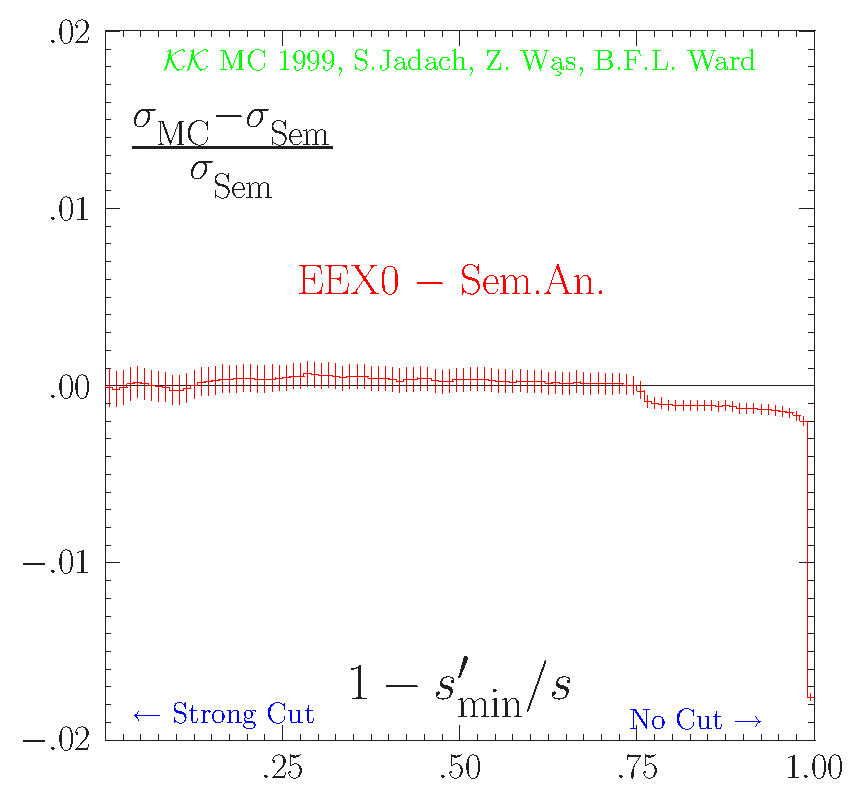
\epsfig{file=chi-mcan-O0dif-vmax1.eps,width=37mm,height=37mm}
}}\end{picture}
%
\begin{picture}(37,37)
\put(30,30){\makebox(0,0)[lb]{\Color{Magenta}(b)}}
\put(-1, 0){\makebox(0,0)[lb]{
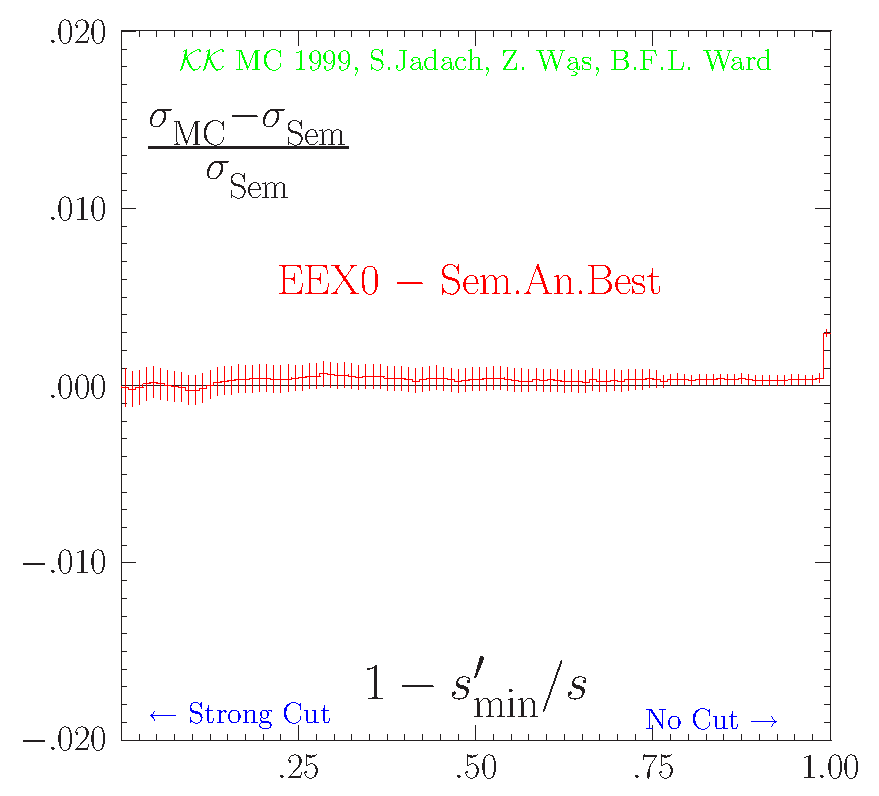
\epsfig{file=chi-mcan-O0tech-vmax1.eps,width=37mm,height=37mm}
}}\end{picture}
%
\end{center}
{\scriptsize
CONCLUSIONS: For the
{\Color{Red}   Born-like  $(M_Z\!+\!\Gamma_Z\!<\!\sqrt{s'}\!<\!\sqrt{s})$},\\
{\Color{Blue}  Z radiative return    $(10GeV\!<\!\sqrt{s'}\!<\!\sqrt{s})$} and\\ 
{\Color{PineGreen} total            $(2m_\mu\!<\!\sqrt{s'}\!<\!\sqrt{s})$}, cross section
using plot (b),\\
we quote technical precision:
\fbox{{\Color{Red} 0.2\%}, {\Color{Blue} 0.2\%} and {\Color{PineGreen} 0.3\%}}
}
%-----------------------------------------------------------
\vfill
\end{slide*}   %%%
%%%%%%%%%%%%%%%%%%


%%%%%%%%%%%%%%%%%%%%%%%%%%%%%%%%%%%%%%%%%%%%%%%%%%%%%%%%%%%%%%%%%%%%%%%%%%%%%
%%%%%%%%%%%%%%%%%%%%%%%%%%%%%%%%%%%%%%%%%%%%%%%%%%%%%%%%%%%%%%%%%%%%%%%%%%%%%
%%%%%%%%%%%%%%%%%%%%%%%%%%%%%%%%%%%%%%%%%%%%%%%%%%%%%%%%%%%%%%%%%%%%%%%%%%%%%
                                                         %%%%%%%%%%%%%%%%%%%%
\begin{slide*}
\titbox{{\small\Color{Magenta} 
      The best semi-analytical cross-check, EEX class}}

\vspace {-2mm}
{\scriptsize\Color{Blue}
  We examine the difference between  ${\cal KK}$  MC
  with the EEX3 mat.el,\\
\hspace{12mm}  \fbox{EEX3 = \Oeex{1,\alpha,\alpha L,\alpha^2 L^2,\alpha^3 L^3}}\\
  and the best semi-analytical formula EEX3best,\\
\hspace{12mm}  \fbox{EEX3best = \Oeex{1,\alpha,\alpha L,\alpha^2 L^2,
                    {\Color{Red} \alpha^2 L} ,\alpha^3 L^3}}
}
\begin{center}
\setlength{\unitlength}{1mm}
\begin{picture}(55,50)
%#####\put(0,0){\framebox( 55,50){ }}
\put(-2, 00){\makebox(0,0)[lb]{
\epsfig{file=chi_mcan-O3dan.eps,width=55mm,height=50mm}
}}
\end{picture}
\end{center}
%
{\small
CONCLUSIONS: For the
{\Color{Red}   Born-like  $(M_Z\!+\!\Gamma_Z\!<\!\sqrt{s'}\!<\!\sqrt{s})$},\\
{\Color{Blue}  Z radiative return    $(10GeV\!<\!\sqrt{s'}\!<\!\sqrt{s})$} and\\ 
{\Color{PineGreen} total            $(2m_\mu\!<\!\sqrt{s'}\!<\!\sqrt{s})$} cross section
using all previous results,\\
we quote total precision:
\doublebox{{\Color{Red} 0.2\%}, {\Color{Blue} 0.7\%} and {\Color{PineGreen} 1.5\%}}
}\\
{\scriptsize\Color{Maroon}
LIMITATIONS:
Neglected IFI=ISR*FSR interf., light fermion pairs.\\
Does not apply if EEX/YFS exponentiation is NOT used.
}
%-----------------------------------------------------------
\vfill
\end{slide*}   %%%
%%%%%%%%%%%%%%%%%%



                                                         %%%%%%%%%%%%%%%%%%%%
%%%%%%%%%%%%%%%%%%%%%%%%%%%%%%%%%%%%%%%%%%%%%%%%%%%%%%%%%%%%%%%%%%%%%%%%%%%%%

\end{document}
